O remo de assento deslizante � um esporte que faz uso de um barco e dois remos do mesmo tamanho. 
A figura mostra uma das posi��es de uma t�cnica chamada afastamento. 

\begin{figure}[h]
\centering
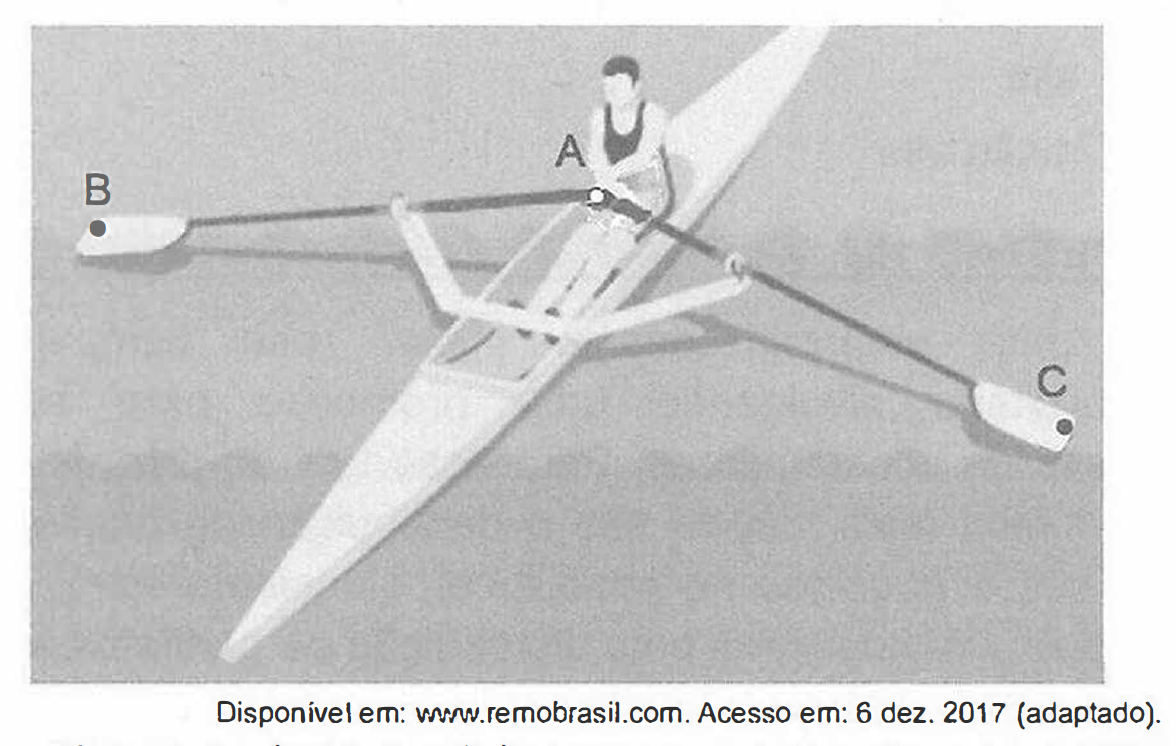
\includegraphics[width=8cm]{../figuras/q165-2018.png}
\end{figure}

Nessa posi��o, os dois remos se encontram no ponto A e suas outras extremidades est�o indicadas pelos pontos B e C. Esses tr�s pontos formam um tri�ngulo ABC cujo �ngulo B�C tem medida de 170�. 
O tipo de tri�ngulo com v�rtices nos pontos A, B e C, no momento em que o remador est� nessa posi��o, � 
\begin{enumerate}
\item[a)]ret�ngulo escaleno
\item[b)] acut�ngula escaleno
\item[c)] acut�ngulo is�sceles
\item[d)]obtus�ngulo escaleno
\item[e)]obtus�ngulo is�sceles.
\end{enumerate}